\section{Model}
The model was created in Siemens NX. Each aerodynamic element has been optimized firstly in 2D, next in 3D. 


\begin{figure}[h!]
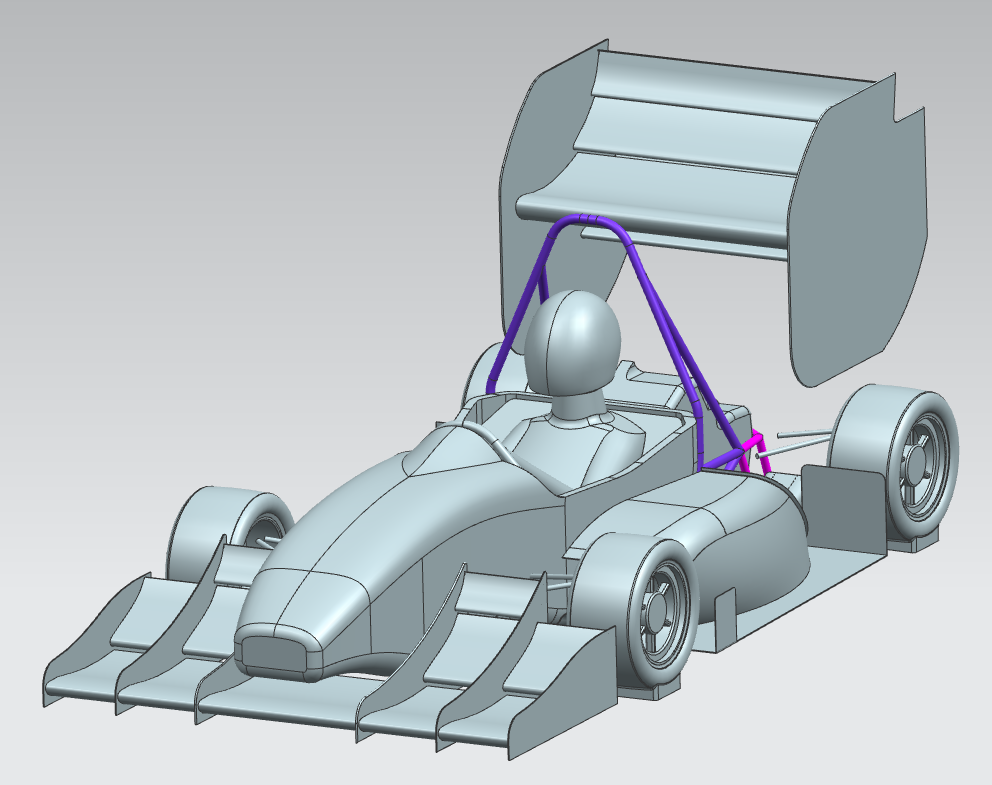
\includegraphics[width=\textwidth]{img/final}
\caption{WUT3 aerodynamics model}
%\label{fig:boat1}
\end{figure}



\section{Mesh}
The mesh was created in Ansys Mesher. It was very difficult to generate good quality mesh, because of complex geometry. Minimum Orthogonal Quality of the mesh is about 7e-02.

It is worth to mention that the mesh has to be export in ASCII format. OpenFoam is working on ASCII and it does not read the mesh wrote in binary. 

Firstly, the mesh was created with boundary layer, which improve calculations precision near walls. Unfortunately, quality of the mesh getting worse with boundary layer and OpenFoam could not calculate this. The residuals and forces reached large values. In this case Fluent was better than OpenFoam, because it made calculations and results was quite good.

In external flow calculations very good option is polyhedral mesh, which can be made in OpenFoam with command polyDualMesh. 

\section{Solver}
For this calculation MotorBike tutorial was adopted. It use incompressible simpleFoam solver and k-omega SST turbulence model which is the best option for external flows around cars.

\section{Step by step}


\subsection{Generate mesh}
As mentioned, the mesh was export in ASCII Fluent Mesh format (.msh) and copied to case folder.


\subsection{fluent3DMeshToFoam}
This command converts Fulent mesh to OpenFoam's format and creates polyMesh folder in constant. There are all parameters of mesh, for example boundaries, which are import with mesh's named selection.


\subsection{Boundary condition}
This step is to adapt boundary conditions in time 0 to right case. In the case, inlet velocity magnitude is $15\frac{m}{s}$. Of course on road is moving wall condition and on wheels are rotating wall condition.


\subsection{Forces and Coefficients}
Very important for car aerodynamics are forces and coefficients (Cx and Cl). OpenFoam can calculate they. It needs special file named forces in system folder. It looks like this:
\begin{figure}[h!]
\begin{center}
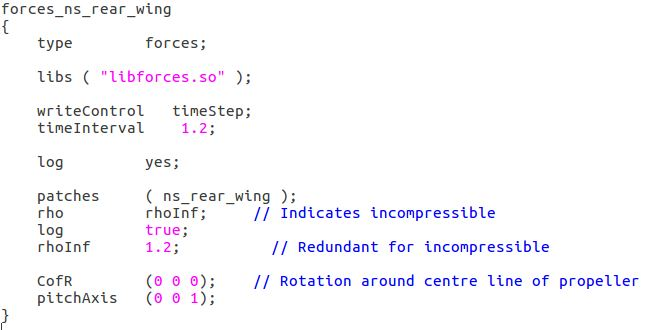
\includegraphics[width=9cm]{img/forces}
\caption{A part of code of forces file}
\end{center}
\end{figure}

The forces are collected from all car's patches. In result OpenFoam create file with forces and moments in all directions.


\subsection{Convert mesh to polyhedral}
Instead of tetrahedral mesh will be used polyhedral mesh, which has less elements, and calculations are more stable. From 15mln elements it was made 3mln. 

polyDualMesh is using to convert mesh to polyhedral. There is one argument - minimum angle between normals to cell's faces. In this calculation it is 30 degrees. Also it should be used options: -overwrite and -doNotPreserveFaceZones. First one (optional), overwrite new mesh in time 0, which is  comfortable. Second delete old faces from mesh. It is necessarily to correct work.

\begin{figure}[h!]
	\centering
    \begin{subfigure}[b]{0.46\linewidth}
    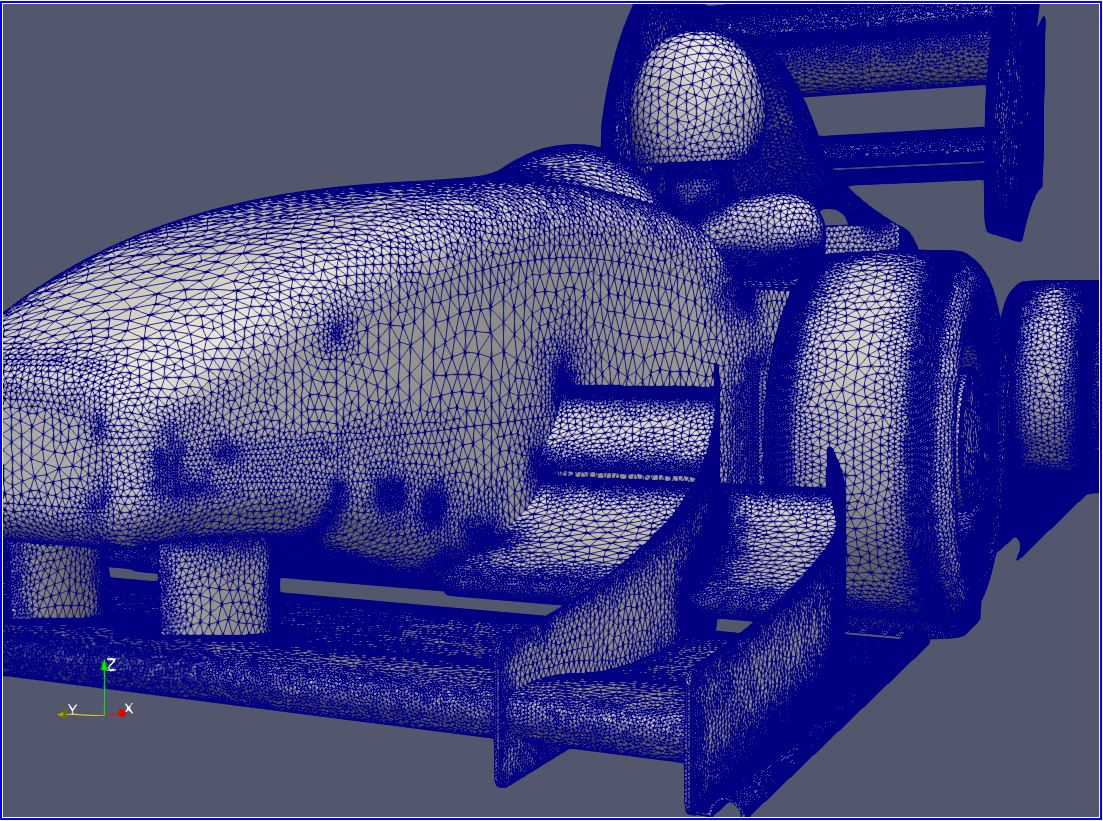
\includegraphics[width=\textwidth]{tetra.JPG}
    \caption{Tetrahedral mesh}
    \end{subfigure}
    
    \begin{subfigure}[b]{0.46\textwidth}
    	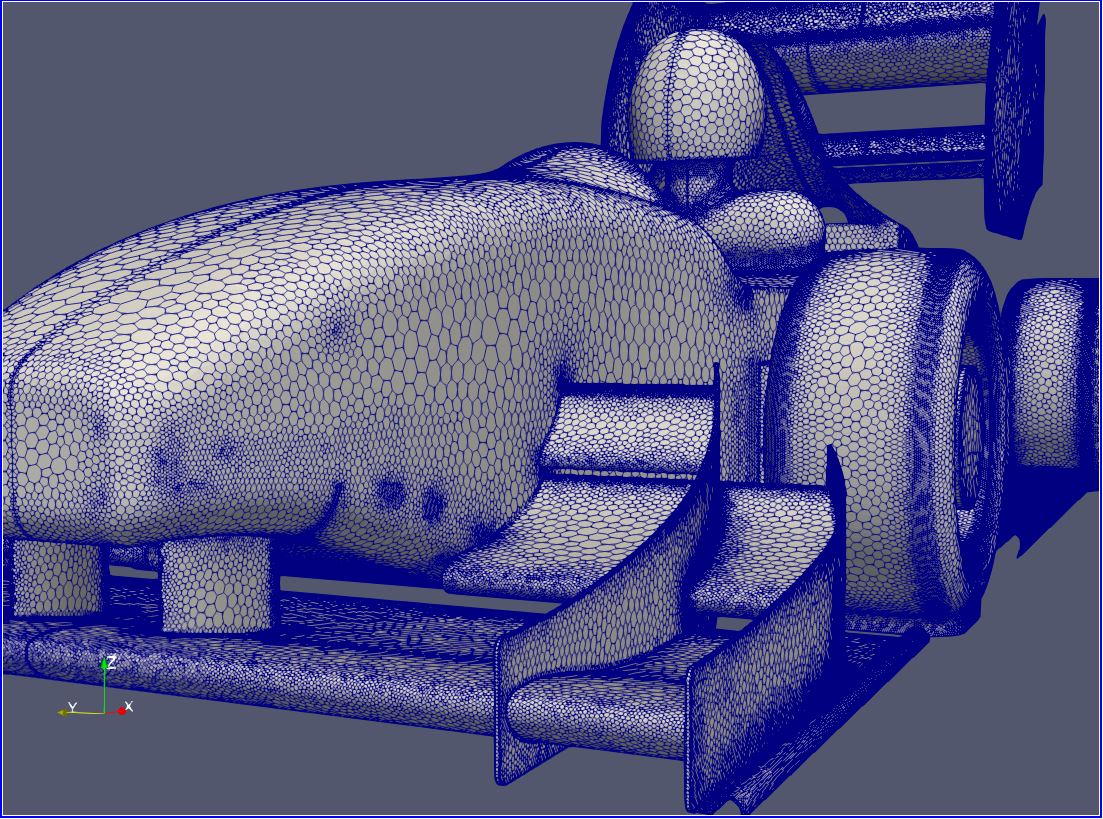
\includegraphics[width=\textwidth]{polyhedra.JPG}
        \caption{Polyhedral mesh}
    \end{subfigure}
    \begin{subfigure}[b]{0.46\textwidth}
    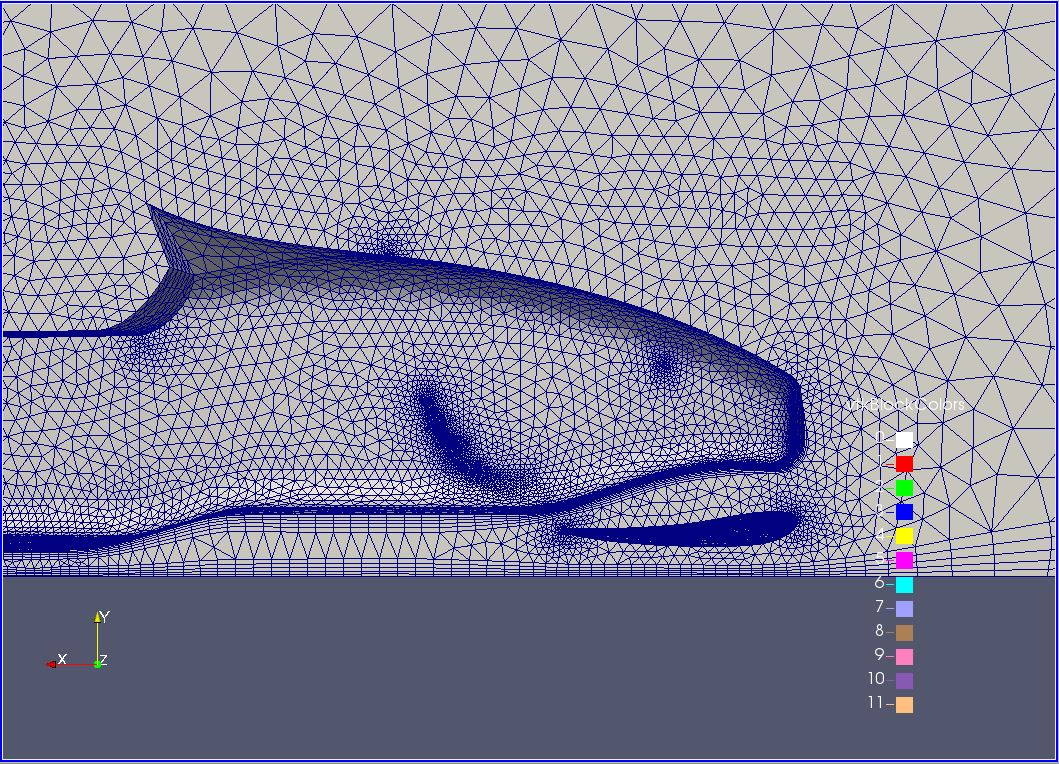
\includegraphics[width=\textwidth]{tetra2.JPG}
    \caption{Tetrahedral mesh}
    \end{subfigure}
    \begin{subfigure}[b]{0.46\textwidth}
    	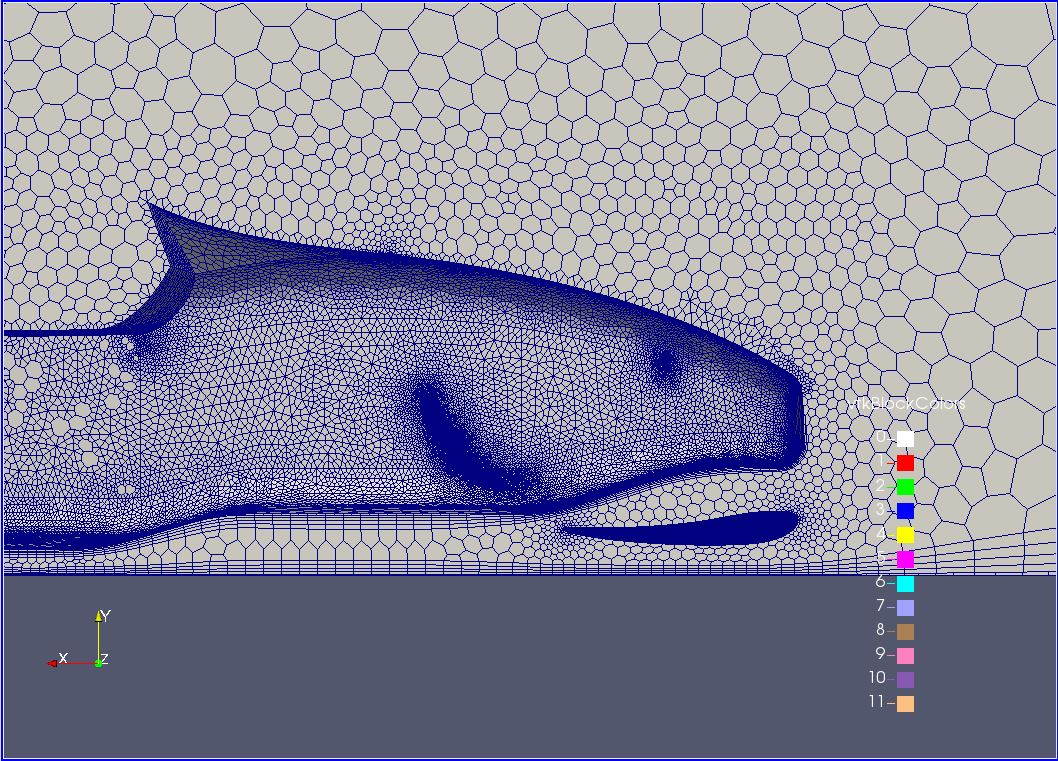
\includegraphics[width=\textwidth]{polyhedra2.JPG}
        \caption{Polyhedral mesh}
    \end{subfigure}
    \caption{Comparison both tetrahedral and polyhedral meshes}
\end{figure}


\subsection{Parallel calculations}
Calculation was carried out on 32 cores, on four EC2 instances. The instances have been merged to cluster. Scotch decompose method has been chosen. 

\subsection{Calculations}
There was 360 time steps and it was enough to stabilize forces and getting good accuracy.